%%%%%%%%%%%%%%%%%%%%%%%%%%%%%%%%%%%%%%%%%
% Jacobs Landscape Poster
% LaTeX Template
% Version 1.0 (29/03/13)
%
% Created by:
% Computational Physics and Biophysics Group, Jacobs University
% https://teamwork.jacobs-university.de:8443/confluence/display/CoPandBiG/LaTeX+Poster
%
% Further modified by:
% Nathaniel Johnston (nathaniel@njohnston.ca)
%
% This template has been downloaded from:
% http://www.LaTeXTemplates.com
%
% License:
% CC BY-NC-SA 3.0 (http://creativecommons.org/licenses/by-nc-sa/3.0/)
%
%%%%%%%%%%%%%%%%%%%%%%%%%%%%%%%%%%%%%%%%%

%----------------------------------------------------------------------------------------
%	PACKAGES AND OTHER DOCUMENT CONFIGURATIONS
%----------------------------------------------------------------------------------------

\documentclass[final]{beamer}

\usepackage[scale=1.24]{beamerposter} % Use the beamerposter package for laying out the poster

% -----PACKAGES
%\usepackage[shortend,titlenumbered]{algorithm2e}
%\usepackage{algorithmic}
%\usepackage[plain]{algorithm}
\usepackage{multicol}
\usepackage{color}
\usepackage{multirow}
\usepackage{fancybox}
%\usepackage{index}
\usepackage{varioref}
\usepackage{psfrag}
\usepackage{epsfig}
\usepackage{boxedminipage}
\usepackage{graphicx}
\usepackage{rotating}
\usepackage{amsmath}
\usepackage{amssymb}
%\usepackage{amsfont}
\usepackage{latexsym}
\usepackage{alltt}
%\usepackage[small,bf]{caption}
\usepackage{url}
%\usepackage{citesort}
%\usepackage{crop}
\usepackage{array}
\usepackage{subfigure}
\usepackage{dcolumn}

% -----SETLENGTH
%\setlength{\captionmargin}{20pt} 

% -----NEWCOMMANDS
\newcommand{\nc}{\newcommand}
\nc{\mathsm}[1]{\text{\small{$#1$}}}
\nc{\ubar}[1]{\underset{-}{#1}}
\nc{\optype}{\textrm}
\nc{\EQ}[1]{(\ref{eq:#1})}
\nc{\TAB}[1]{\ref{tab:#1}}
\nc{\FIG}[1]{\ref{fig:#1}}
\nc{\SEC}[1]{\ref{sec:#1}}
\nc{\ALG}[1]{\ref{alg:#1}}
\nc{\CHAP}[1]{\ref{chap:#1}}
\nc{\mtrx}[1]{\boldsymbol{\mathbf{#1}}}
\nc{\vctr}[1]{\boldsymbol{\mathbf{#1}}}
\nc{\grad}{\mbox{\boldmath$\nabla$}}
\nc{\gradient}{\textsl{grad}\,}
\nc{\hessian}{\textsl{grad\,}^2}
\nc{\ii}{\iota}
\nc{\dd}{d}
\nc{\ee}{\mathrm{e}}
\nc{\pdiv}[2]{\partial{#1}/\partial{#2}}
\nc{\dpdiv}[2]{\displaystyle{\frac{\partial{#1}}{\partial{#2}}}}
\nc{\ddiv}[2]{\displaystyle{\frac{\dd{#1}}{\dd{#2}}}}
\nc{\inpr}{\hspace{-1pt}\cdot\hspace{-1pt}}
\nc{\IR}{\mathbb{R}}
\nc{\IN}{\mathbb{N}}
\nc{\IZ}{\mathbb{Z}}
\nc{\IC}{\mathbb{C}}
\nc{\half}{\frac{1}{2}}
\nc{\shalf}{\scriptstyle{\half}} 
\nc{\ds}[1]{\displaystyle{#1}}
\nc{\ts}[1]{\textstyle{#1}}
\nc{\sign}{\optype{sign}}
\nc{\spr}{\optype{spr}}
\nc{\dist}{\optype{dist}}
\nc{\rank}{\optype{rank}}
\nc{\codim}{\optype{codim}}
\nc{\supp}{\optype{supp}}
\nc{\diag}{\optype{diag}}
\nc{\meas}{\optype{meas}}
\nc{\cond}{\optype{cond}}
\nc{\kernel}{\optype{kernel}}
\nc{\spa}{\optype{span}}
\nc{\order}{\mathcal{O}}
\nc{\Fr}{\mathrm{Fr}}
\nc{\Rey}{\mathrm{Re}}
\nc{\Ord}{O}
\nc{\ord}{o}
\nc{\st}{\:{:}\:}
\nc{\closure}[1]{\overline{#1}}
\nc{\emin}[1]{\emph{#1}\index{#1}\/}
\nc{\rmin}[1]{#1\index{{}@{#1}}}
\nc{\Laplace}{\Delta}
\nc{\ie}{i.e.}
\nc{\eg}{e.g.}
%\nc{\union}{\cup}
\nc{\Union}{\bigcup}
\nc{\lf}[1]{\mathsf{#1}}
\nc{\dbar}[1]{\bar{\bar{#1}}}
\nc{\ul}[1]{\underline{#1}}
\nc{\hpt}{\hspace{0.5pt}}
\nc{\E}[1]{\times{}10^{#1}}
\nc{\inp}[2]{\langle{#1},{#2}\rangle}
\nc{\tmpcommand}{}

% -----RENEWCOMMANDS
\renewcommand{\baselinestretch}{1}
\renewcommand{\exp}{\optype{exp}\,}
\renewcommand{\cosh}{\optype{cosh}\,}
\renewcommand{\tanh}{\optype{tanh}\,}
\renewcommand{\sinh}{\optype{sinh}\,}
\renewcommand{\div}[1]{\optype{div}\,{#1}}
\renewcommand{\half}{\mbox{$\frac{1}{2}$}}
%\renewcommand{\descriptionlabel}[1]{\hspace{\labelsep}\emph{#1}}

% -----ETC
\raggedbottom


\DeclareMathOperator{\curl}{\bf curl}
\DeclareMathOperator{\rot}{\rm curl}
\DeclareMathOperator{\divv}{\rm div}
\newcommand{\tro}{\gamma_0}
\newcommand{\trt}{\gamma_{\sft}}
\newcommand{\trn}{\gamma_{\sfn}}

\newcommand{\PT}{{\partial T}}
\newcommand{\bbN}{{\mathbb{N}}}
\newcommand{\bbP}{{\mathbb{P}}}

\newcommand{\scC}{{\mathscr{C}}}
\newcommand{\caD}{{\mathcal{D}}}
\newcommand{\caL}{{\mathcal{L}}}

\newcommand{\sfe}{{\mathsf{e}}}
\newcommand{\sff}{{\mathsf{f}}}
\newcommand{\sft}{{\boldsymbol{\mathsf{t}}}}
\newcommand{\sfn}{{\boldsymbol{\mathsf{n}}}}

%   Common caligraphic abbrevs
\newcommand{\BB}{\mathcal{B}}
\newcommand{\CC}{\mathcal{C}}
\newcommand{\DD}{\mathcal{D}}
\newcommand{\EE}{\mathcal{E}}
\newcommand{\FF}{\mathcal{F}}
\newcommand{\GG}{\mathcal{G}}
\newcommand{\II}{\mathcal{I}}
\newcommand{\JJ}{\mathcal{J}}
\newcommand{\KK}{\mathcal{K}}
\newcommand{\LL}{\mathcal{L}}
\newcommand{\OO}{\mathcal{O}}
\newcommand{\QQ}{\mathcal{Q}}
\newcommand{\RR}{\mathcal{R}}
\newcommand{\TT}{\mathcal{T}}


 %% JAY'S PREAMBLE
 %%========================

%   Math symbol definitions
\def\d{\partial}
%\newsymbol\lee 132E
\newcommand{\union}{\mathop{\bigcup}}
\newcommand{\intersect}{\mathop{\bigcap}}
\newcommand{\binomial}[2]{\ensuremath{
		\begin{pmatrix}{#1}\\{#2}\end{pmatrix}}}
\newcommand{\smallbinomial}[2]{\ensuremath{
		(\begin{smallmatrix}{#1}\\{#2}\end{smallmatrix})}}
\newcommand{\tang}[1]{\ensuremath{{#1}_{\intercal}}} % can use \top
						     % also
\newcommand{\hypergeom}[2]{\ensuremath{\sideset{_{#1}}{_{#2}}{\mathop{F}}}}
%   Difficult names
\newcommand{\Babuska}{Babu{\v{s}}ka}       % Remember: Usage is \Babuska\
\newcommand{\Cea}{C{\'e}a}                 % with trailing `\' to give space
\newcommand{\Poincare}{Poincar{\'{e}}}     % when needed, but when ending
\newcommand{\Nedelec}{N{\'{e}}d{\'{e}}lec} % sentence use \Babuska.
\newcommand{\Frechet}{Fr{\'{e}}chet}
\newcommand{\Muller}{M{\"u}ller}
\newcommand{\LHospital}{L'H{\^{o}}spital}
%   Bold and beautiful
\newcommand{\ba}{{\boldsymbol{a}}}
\newcommand{\bA}{\boldsymbol{A}}
\newcommand{\balpha}{{\boldsymbol{\alpha}}}
\newcommand{\bB}{{\boldsymbol{B}}}
\newcommand{\bb}{{\boldsymbol{b}}}
\newcommand{\bbeta}{{\boldsymbol{\beta}}}
\newcommand{\etab}{{\boldsymbol{\eta}}}
\newcommand{\bC}{{\boldsymbol{C}}}
\newcommand{\bc}{{\boldsymbol{c}}}
\newcommand{\bD}{{\boldsymbol{D}}}
\newcommand{\bd}{{\boldsymbol{d}}}
\newcommand{\db}{{\boldsymbol{\d}}}
\newcommand{\bdelta}{{\boldsymbol{\delta}}}
\newcommand{\bDelta}{{\boldsymbol{\Delta}}}
\newcommand{\beps}{{\boldsymbol{\varepsilon}}}
\newcommand{\be}{{\boldsymbol{e}}}
\newcommand{\bg}{{\boldsymbol{g}}}
\newcommand{\bm}{{\boldsymbol{m}}}
\newcommand{\bn}{{\boldsymbol{n}}}
\newcommand{\bN}{{\boldsymbol{N}}}
\newcommand{\bp}{{\boldsymbol{p}}}
\newcommand{\bpsi}{{\boldsymbol{\psi}}}
\newcommand{\bq}{{\boldsymbol{q}}}
\newcommand{\bxi}{{\boldsymbol{\xi}}}
\newcommand{\bE}{{\boldsymbol{E}}}
\newcommand{\bF}{{\boldsymbol{F}}}
\newcommand{\bh}{{\boldsymbol{h}}}
\newcommand{\bH}{{\boldsymbol{H}}}
\newcommand{\bI}{{\boldsymbol{I}}}
\newcommand{\bj}{{\boldsymbol{j}}}
\newcommand{\bJ}{{\boldsymbol{J}}}
\newcommand{\bK}{{\boldsymbol{K}}}
\newcommand{\bk}{{\boldsymbol{k}}}
\newcommand{\bll}{{\boldsymbol{\ell}}}
\newcommand{\bL}{{\boldsymbol{L}}}
\newcommand{\blambda}{{\boldsymbol{\lambda}}}
\newcommand{\bmu}{{\boldsymbol{\mu}}}
\newcommand{\bM}{{\boldsymbol{M}}}
\newcommand{\bomega}{{\boldsymbol{\omega}}}
\newcommand{\bP}{{\boldsymbol{P}}}
\newcommand{\bphi}{{\boldsymbol{\phi}}}
\newcommand{\bQ}{{\boldsymbol{Q}}}
\newcommand{\bG}{{\boldsymbol{G}}}
\newcommand{\bu}{{\boldsymbol{u}}}
\newcommand{\bU}{{\boldsymbol{U}}}
\newcommand{\bV}{{\boldsymbol{V}}}
\newcommand{\bX}{{\boldsymbol{X}}}
\newcommand{\bv}{{\boldsymbol{v}}}
\newcommand{\bw}{{\boldsymbol{w}}}
\newcommand{\bW}{{\boldsymbol{W}}}
\newcommand{\bR}{{\boldsymbol{R}}}
\newcommand{\br}{{\boldsymbol{r}}}
\newcommand{\bS}{{\boldsymbol{S}}}
\newcommand{\bT}{{\boldsymbol{T}}}
\newcommand{\btau}{{\boldsymbol{\tau}}}
\newcommand{\bt}{{\boldsymbol{t}}}
\newcommand{\bx}{{\boldsymbol{x}}}
\newcommand{\by}{{\boldsymbol{y}}}
\newcommand{\bz}{{\boldsymbol{z}}}
\newcommand{\bzero}{{\boldsymbol{0}}}
\newcommand{\bZ}{{\boldsymbol{Z}}}
%   Common scalar fields
\newcommand{\RRR}{\mathbb{R}}
\newcommand{\CCC}{\mathbb{C}}
\newcommand{\ZZZ}{\mathbb{Z}}
\newcommand{\NNN}{\mathbb{N}}
%   Differential operators
\newcommand{\dive}{\mathop\mathrm{div}}
%\newcommand{\grad}{\ensuremath{\mathop{{\bf{grad}}}}}
%\newcommand{\curl}{{\ensuremath\mathop{\mathbf{curl}\,}}}
\newcommand{\Curl}{ {\bf Curl}}
\newcommand{\dx}{\ensuremath{\mathrm{d}x}}
\newcommand{\dy}{\ensuremath{\mathrm{d}y}}
\newcommand{\dr}{\ensuremath{\mathrm{d}r}}
\newcommand{\dR}{\ensuremath{\mathrm{d}R}}
\newcommand{\drho}{\ensuremath{\mathrm{d}\rho}}
\newcommand{\dz}{\ensuremath{\mathrm{d}z}}
\newcommand{\dzeta}{\ensuremath{\mathrm{d}\zeta}}
%   Wordy math symbols
\newcommand{\card}{\ensuremath{\mathop\mathrm{card}}}
%\newcommand{\diag}{\ensuremath{\mathop\mathrm{diag}}}
\newcommand{\diam}{\ensuremath{\mathop\mathrm{diam}}}
%\newcommand{\dist}{\mathop\mathrm{dist}}
\newcommand{\Ker}{\mathop\mathrm{Ker}}
\newcommand{\Range}{\mathop\mathrm{Range}}
%\newcommand{\rank}{\mathop\mathrm{rank}}
%\newcommand{\meas}{\mathop\mathrm{meas}}
\newcommand{\Forall}{\quad\text{for all }}
%\newcommand{\supp}{\mathop\mathrm{supp}}
\newcommand{\Span}{\mathop\mathrm{Span}}
\newcommand{\Hdiv}[1]{\bH(\dive,#1)}
%\newcommand{\Hcurl}[1]{\bH(\curl,#1)}
%   Common caligraphic abbrevs
%\newcommand{\BB}{\mathcal{B}}
%\newcommand{\CC}{\mathcal{C}}
%\newcommand{\DD}{\mathcal{D}}
%\newcommand{\EE}{\mathcal{E}}
%\newcommand{\FF}{\mathcal{F}}
%\newcommand{\GG}{\mathcal{G}}
%\newcommand{\II}{\mathcal{I}}
%\newcommand{\JJ}{\mathcal{J}}
%\newcommand{\KK}{\mathcal{K}}
%\newcommand{\LL}{\mathcal{L}}
%\newcommand{\OO}{\mathcal{O}}
%\newcommand{\QQ}{\mathcal{Q}}
%\newcommand{\RR}{\mathcal{R}}
%\newcommand{\TT}{\mathcal{T}}
%   Variations on standard symbols
\newcommand{\veps}{\varepsilon}
\newcommand{\vlam}{\varLambda}
\newcommand{\vpi}{\varPi}
\newcommand{\vPi}{\boldsymbol{\varPi}}
\newcommand{\vsig}{\varSigma}
\newcommand{\vbt}{\boldsymbol{\varTheta}}
\newcommand{\vPsi}{\boldsymbol{\varPsi}}
%\newcommand{\ii}{\hat{\imath}}
%   Innerproducts, norms, etc
\newcommand{\ntrip}[1]{|\!|\!| {#1} |\!|\!|}
\newcommand{\ip}[1]{\langle {#1} \rangle}
%   Utilities
\newcommand{\blnk}{\underline{\hspace{3cm}}\;}
\newcommand{\marg}[1]{\marginpar{\tiny{\framebox{\parbox{1.7cm}{#1}}}}}
\newcommand{\degreeC}[1]{\ensuremath{{#1\,}^\circ\!\text{C}}}
                        % try also  \textcelsius of textcomp package
%   Trademarked names \texttrademark, \textregistered
\newcommand{\matlab}{MATLAB\textregistered\renewcommand{\matlab}{MATLAB}}
\newcommand{\femlab}{FEMLAB\textregistered\renewcommand{\femlab}{FEMLAB}}

%   Style preferences
\renewcommand{\thefootnote}{\fnsymbol{footnote}} % Use symbols instead of
						 % numbers for footnotes
						 

\newcommand{\Eg}{\EE^\mathrm{grad}}
\newcommand{\Ec}{\boldsymbol{\EE}^\mathrm{curl}}
\newcommand{\Ed}{\boldsymbol{\EE}^\mathrm{div}}


\newcommand{\bfdu}{\mbox{\boldmath $\delta u$}}
\newcommand{\bfdv}{\mbox{\boldmath $\delta v$}}
\newcommand{\du}{{\delta u}}
\newcommand{\dv}{{\delta v}}
\newcommand{\bfnabt}{\widetilde{\bfnab}}
\newcommand{\bfepst}{\widetilde{\bfeps}}

\graphicspath{{../Figures/}}
\usepackage{bbding}
\usetheme{confposter} % Use the confposter theme supplied with this template
\usepackage{exscale}

\setbeamercolor{block title}{fg=utorange,bg=white} % Colors of the block titles
\setbeamercolor{block body}{fg=black,bg=white} % Colors of the body of blocks
\setbeamercolor{block alerted title}{fg=black,bg=utsecgreen} % Colors of the highlighted block titles
\setbeamercolor{block alerted body}{fg=black,bg=dblue!10} % Colors of the body of highlighted blocks

% \setbeamercolor{block title}{fg=ngreen,bg=white} % Colors of the block titles
% \setbeamercolor{block body}{fg=black,bg=white} % Colors of the body of blocks
% \setbeamercolor{block alerted title}{fg=white,bg=dblue!70} % Colors of the highlighted block titles
% \setbeamercolor{block alerted body}{fg=black,bg=dblue!10} % Colors of the body of highlighted blocks
% Many more colors are available for use in beamerthemeconfposter.sty

%-----------------------------------------------------------
% Define the column widths and overall poster size
% To set effective sepwid, onecolwid and twocolwid values, first choose how many columns you want and how much separation you want between columns
% In this template, the separation width chosen is 0.024 of the paper width and a 4-column layout
% onecolwid should therefore be (1-(# of columns+1)*sepwid)/# of columns e.g. (1-(4+1)*0.024)/4 = 0.22
% Set twocolwid to be (2*onecolwid)+sepwid = 0.464
% Set threecolwid to be (3*onecolwid)+2*sepwid = 0.708

\newlength{\sepwid}
\newlength{\onecolwid}
\newlength{\twocolwid}
\newlength{\threecolwid}
\setlength{\paperwidth}{48in} % A0 width: 46.8in
\setlength{\paperheight}{36in} % A0 height: 33.1in
\setlength{\sepwid}{0.024\paperwidth} % Separation width (white space) between columns
\setlength{\onecolwid}{0.22\paperwidth} % Width of one column
\setlength{\twocolwid}{0.464\paperwidth} % Width of two columns
\setlength{\threecolwid}{0.708\paperwidth} % Width of three columns
\setlength{\topmargin}{-0.5in} % Reduce the top margin size
%-----------------------------------------------------------

\usepackage{graphicx}  % Required for including images

\usepackage{booktabs} % Top and bottom rules for tables

%----------------------------------------------------------------------------------------
%	TITLE SECTION
%----------------------------------------------------------------------------------------
\title{Space-Time DPG for Fluid Problems} % Poster title

\author{Truman Ellis and Leszek Demkowicz} % Author(s)

\institute{Institute for Computational Engineering and Sciences, University of
Texas} % Institution(s)

%----------------------------------------------------------------------------------------

\begin{document}

\addtobeamertemplate{block end}{}{\vspace*{2ex}} % White space under blocks
\addtobeamertemplate{block alerted end}{}{\vspace*{2ex}} % White space under highlighted (alert) blocks

\setlength{\belowcaptionskip}{2ex} % White space under figures
\setlength\belowdisplayshortskip{2ex} % White space under equations

\begin{frame}[t] % The whole poster is enclosed in one beamer frame

\begin{columns}[t] % The whole poster consists of three major columns, the second of which is split into two columns twice - the [t] option aligns each column's content to the top

\begin{column}{\sepwid}\end{column} % Empty spacer column

\begin{column}{\onecolwid} % The first column

%----------------------------------------------------------------------------------------
%	OBJECTIVES
%----------------------------------------------------------------------------------------

% \begin{alertblock}{Objectives}
%
% Lorem ipsum dolor sit amet, consectetur, nunc tellus pulvinar tortor, commodo eleifend risus arcu sed odio:
% \begin{itemize}
% \item Mollis dignissim, magna augue tincidunt dolor, interdum vestibulum urna
% \item Sed aliquet luctus lectus, eget aliquet leo ullamcorper consequat. Vivamus eros sem, iaculis ut euismod non, sollicitudin vel orci.
% \item Nascetur ridiculus mus.
% \item Euismod non erat. Nam ultricies pellentesque nunc, ultrices volutpat nisl ultrices a.
% \end{itemize}
%
% \end{alertblock}

%----------------------------------------------------------------------------------------
%	INTRODUCTION
%----------------------------------------------------------------------------------------

\begin{block}{Introduction}
The discontinuous Petrov-Galerkin method is a novel finite element framework with exceptional stability and adaptivity properties.
The DPG framework can be used to derive stable discretizations of any well-posed variational formulation.
In contrast to many other numerical methods, DPG does not suffer from a pre-asymptotic regime (unstable behavior on coarse meshes).
This means that a simulation can be initiated at the coarsest scale possible while automatic adaptivity resolves solution features 
based on a robust, built-in measure of residual error.
We present preliminary work on a space-time DPG formulation that enables automatic local time stepping and a kind of parallel-in-time integration.
% The discontinuous Petrov-Galerkin method is a novel finite element framework with exceptional stability and adaptivity properties.
% The DPG framework can be used to derive stable discretizations of any well-posed variational formulation 
% and has been successfully applied to problems such as heat conduction, time-harmonic Helmholtz, 
% Maxwell's equations, linear elasticity and plate problems, Stokes flow, and both incompressible and compressible Navier-Stokes.
% In contrast to many other numerical methods, DPG does not suffer from a pre-asymptotic regime (unstable behavior on coarse meshes).
% This means that a simulation can be initiated at the coarsest scale possible while automatic adaptivity resolves solution features 
% based on a robust, built-in measure of residual error.
% DPG is intensely locally compute intensive with significant embarrassingly parallel computations done both pre- and post-global solve.
% We present preliminary work on a space-time DPG formulation that enables automatic local time stepping and a kind of parallel-in-time integration.

% The discontinuous Petrov-Galerkin finite element method has been described as least squares finite ele-
% ments with a twist. The key difference is that least squares methods seek to minimize the residual of the
% solution in the $L^2$ norm, while DPG seeks the minimization in a dual norm realized through the inverse Riesz
% map. 
% Exact mass conservation has been an issue that has plagued least squares finite elements for a long
% time. In this work, we augment our DPG system with Lagrange multipliers in
% order to exactly enforce local conservation. Effectively, this turns our
% minimization problem into a constrained minimization problem. We note that
% standard DPG, while not guaranteed to be conservative, appears to be nearly
% conservative in practice.

\end{block}

%----------------------------------------------------------------------------------------
%	INTRODUCTION
%----------------------------------------------------------------------------------------

\begin{block}{A Minimum Residual Method}

Let $U$ and $V$ be trial and test Hilbert spaces for a well-posed variational
problem $b(u,v)=l(v)$. In operator form this is $Bu=l$, where $B:U\rightarrow
V'$. We seek to minimize the residual for the discrete space $U_h\subset U$:
\[
u_{h} = \underset{w_{h} \in U_{h}} \argmin \,\, \frac{1}{2}
\norm{Bw_{h}-l}_{V'}^{2}
\]
Use the Riesz inverse to minimize in the $V$-norm rather than its dual:
\begin{align*}
\frac{1}{2}&\norm{Bu_h-l}^2_{V'}=\frac{1}{2}\norm{R_V^{-1}(Bu_h-l)}^2_V\\
&=\frac{1}{2}\LRp{R_V^{-1}(Bu_h-l),R_V^{-1}(Bu_h-l)}_V\,.
\end{align*}
First order optimality requires
the G\^ateaux derivative to be zero in all directions $\delta u \in
U_h$, i.e.,
\[
\left(R_V^{-1}(Bu_h-l),R_V^{-1}B\delta u\right)_V = 0, \quad \forall \delta u \in U_h.
\]
By definition of the Riesz operator, this is equivalent to
\begin{equation*}
\LRa{Bu_h-l,R_V^{-1}B\delta u_h}=0\quad\forall\delta u_h\in U_h\,.
\end{equation*}
Identify $v_{\delta u_h}\coloneqq R_V^{-1}B\delta u_h$ as the
optimal test function for trial function $\delta u_h$. This gives us
\begin{equation*}
b(u_h,v_{\delta u_h})=l(v_{\delta u_h}).
\end{equation*}

\end{block}


%----------------------------------------------------------------------------------------

\end{column} % End of the first column

\begin{column}{\sepwid}\end{column} % Empty spacer column


%----------------------------------------------------------------------------------------
%	COLUMN
%----------------------------------------------------------------------------------------
\begin{column}{\onecolwid} % The second column

\begin{block}{Space-Time DPG}

\begin{itemize}
  \item Time stepping techniques are not ideally suited to highly adaptive grids
  \item Space-time FEM proposed as a solution
  \begin{itemize}
    \item[\textcolor{green}{\Checkmark}] Unified treatment of space and time
    \item[\textcolor{green}{\Checkmark}] Local space-time adaptivity (local time stepping)
    \item[\textcolor{green}{\Checkmark}] Parallel-in-time integration
    \item[\textcolor{red}{\XSolidBrush}] Spatially stable FEM methods may not be stable in space-time
    \item[\textcolor{red}{\XSolidBrush}] Need to support higher dimensional problems
  \end{itemize}
  \item DPG provides necessary stability and adaptivity
\end{itemize}
\begin{figure}[b]
\centering
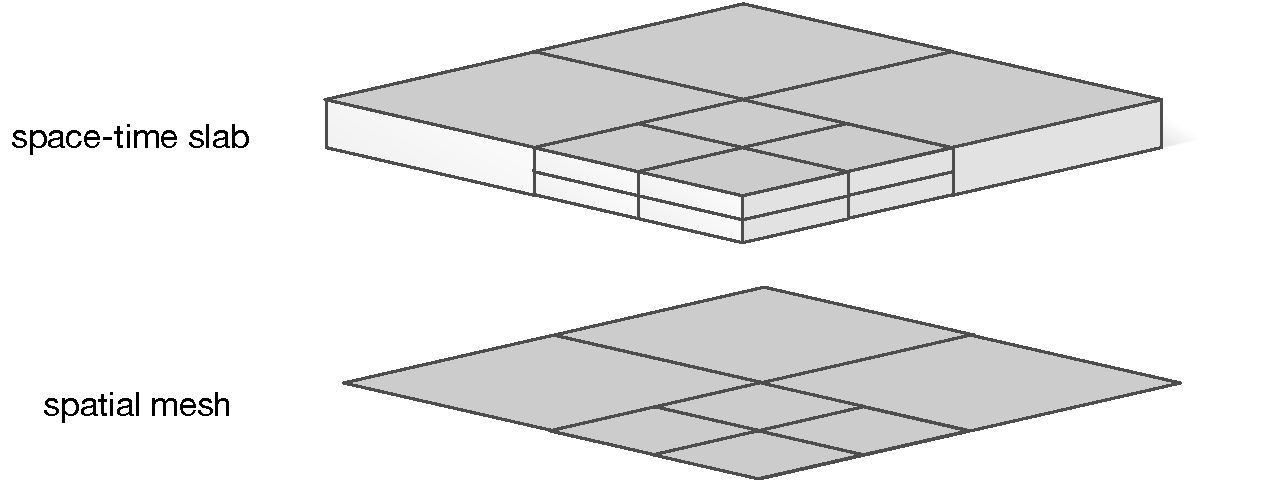
\includegraphics[width=0.8\textwidth]{Schematics/SpaceTimeSchematic}
\end{figure}

\end{block}

\begin{block}{Ultra-Weak Transient Convection-Diffusion}

Start with the strong-form PDE.
\[
\pd{u}{t}+\nabla\cdot(\bfbeta u)-\epsilon\Delta u = g
\]
Rewrite as a system of first-order equations.
\begin{align*}
\frac{1}{\epsilon}\bfsigma-\nabla u&=\boldsymbol0\\
\Divxt\vecttwo{\bfbeta u-\bfsigma}{u}&=g
\end{align*}
Multiply by test functions and integrate by parts over each element, $K$.
% \begin{align*}
% -\LRp{\vecttwo{\bfbeta u-\bfsigma}{u},\nabla_{xt} v}_K\hspace{-1em}+\LRa{(\bfbeta
% u-\bfsigma)\cdot\mathbf{n},v}_{\partial K}&=(g,v)_K\\
% \frac{1}{\epsilon}\LRp{\bfsigma,\bftau}_K+\LRp{u,\nabla\cdot\bftau}_K
% -\LRa{u,\tau_n}_{\partial K}&=0
% \end{align*}
Declare traces and fluxes to be independent unknowns and incorporate boundary
conditions to obtain the final variational formulation.
\begin{align*}
&\frac{1}{\epsilon}(\bfsigma,\bftau)_K
+(u,\nabla\cdot\bftau)_K
-\LRa{\hat u,\tau_n}_{\partial K}\\
&-\LRp{\vecttwo{\bfbeta u-\bfsigma}{u},\nabla_{xt} v}_K+\LRa{\hat f,v}_{\partial K}
=(g,v)_K
\end{align*}
\begin{figure}
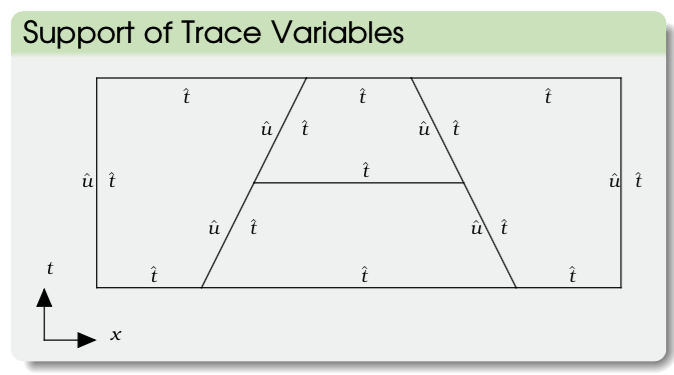
\includegraphics[width=0.7\linewidth]{figs/TraceSupport.png}
\end{figure}
\end{block}

%----------------------------------------------------------------------------------------

\end{column} % End second column

\begin{column}{\sepwid}\end{column} % Empty spacer column

\begin{column}{\onecolwid} % The third column


\begin{block}{Sod Shock-Tube Results}

Extension to other fluid problems like compressible Navier-Stokes
equation is straightforward. 

Sod and Noh results computed with small physical viscosity ($10^{-5}$ and $10^{-3}$ respectively), 
but no shock capturing or artificial viscosity.
\begin{figure}
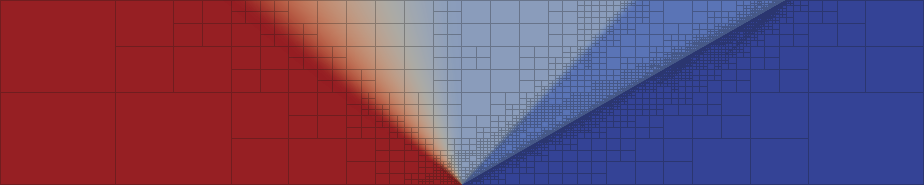
\includegraphics[width=\linewidth]{Sod/MinNSDecoupled1e-5/mesh15.png}\\
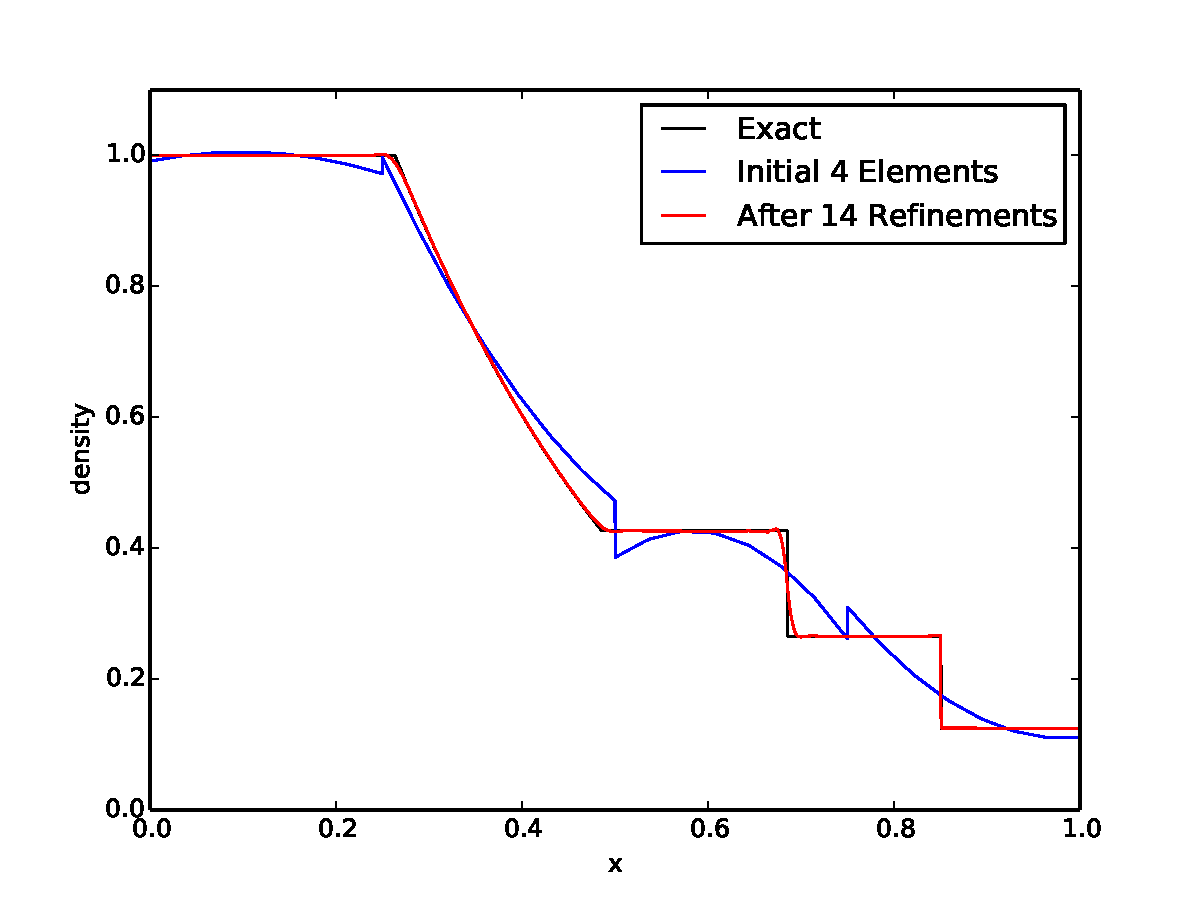
\includegraphics[width=0.8\linewidth]{figs/SodComparison.pdf}\\
% 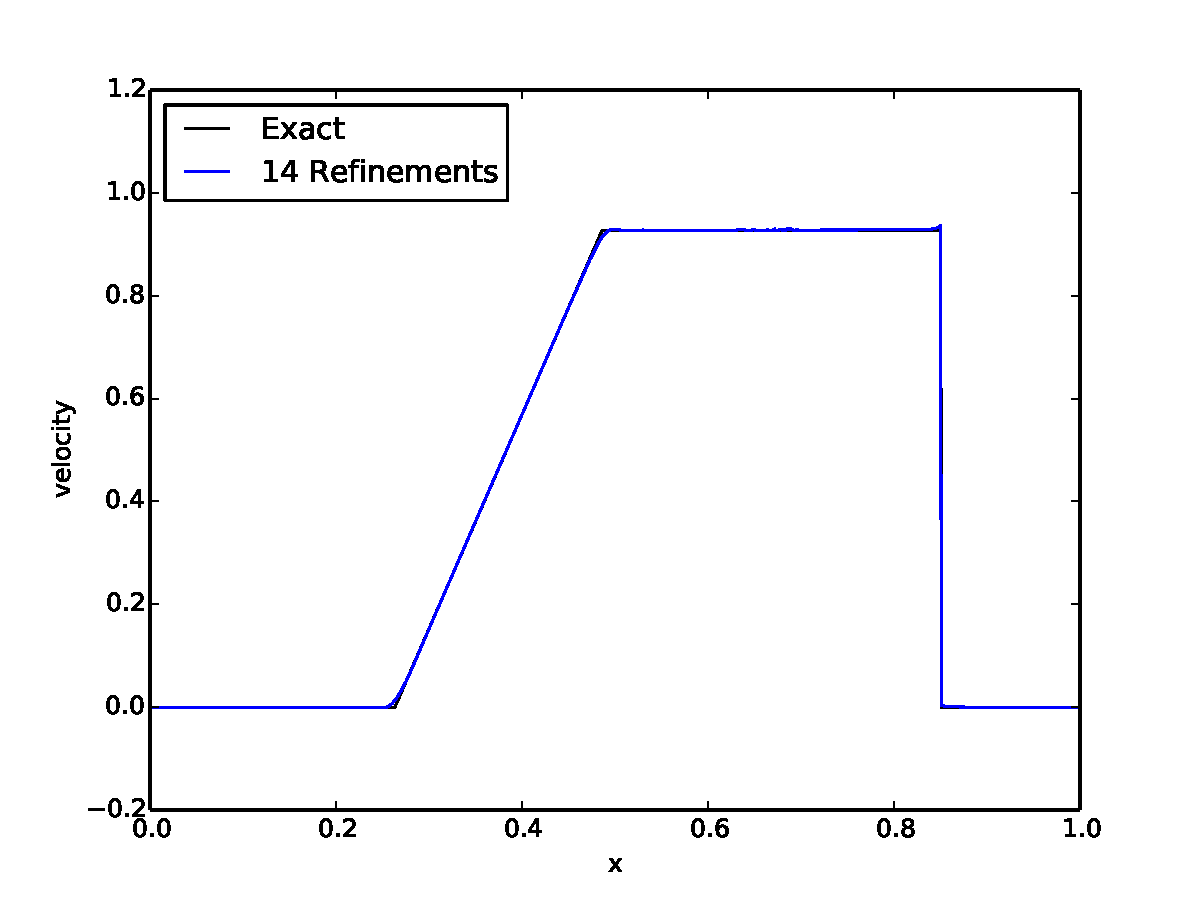
\includegraphics[width=0.8\linewidth]{Sod/MinNSDecoupled1e-5/vel15.pdf}\\
% 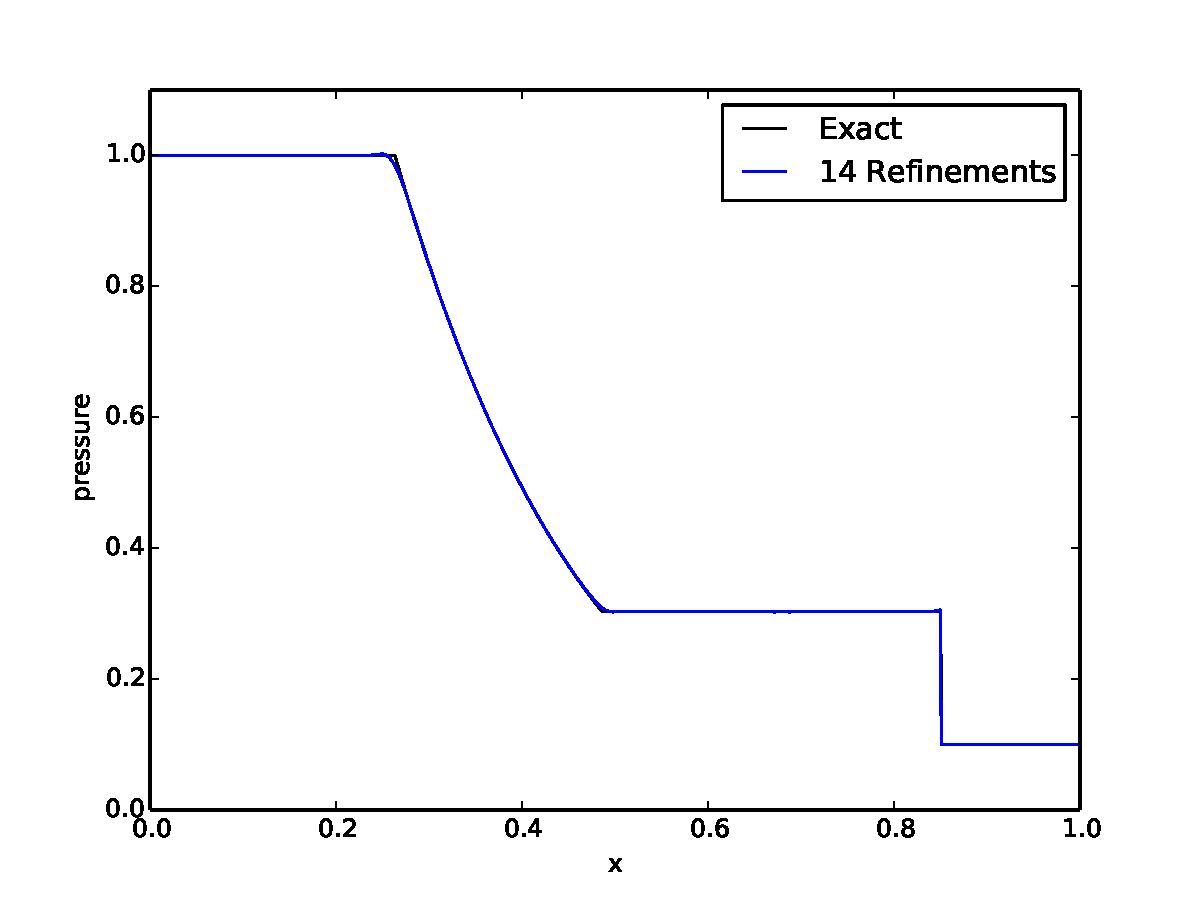
\includegraphics[width=0.8\linewidth]{Sod/MinNSDecoupled1e-5/pres15.pdf}\\
\end{figure}
\end{block}

\begin{block}{Noh Implosion Results}
Computed with a sequence of 4 time slabs.
\begin{figure}
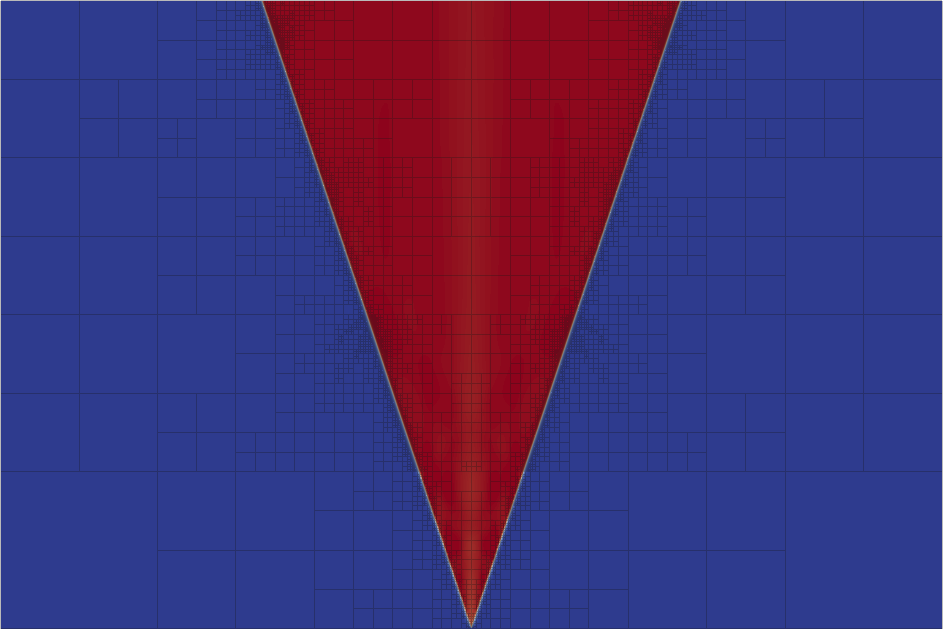
\includegraphics[width=0.8\linewidth]{Noh/MinNSDecoupled/mesh9.png}\\
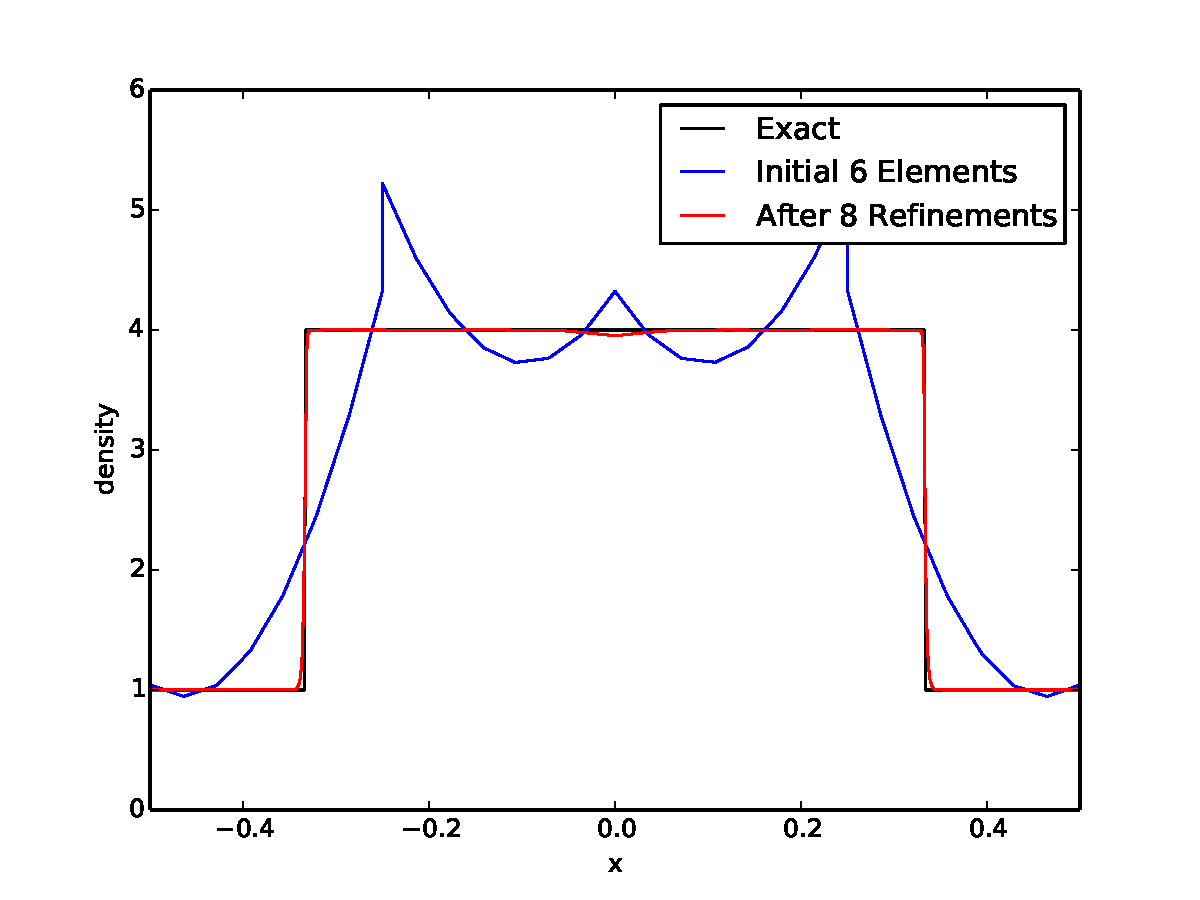
\includegraphics[width=0.8\linewidth]{figs/NohComparison.pdf}\\
\end{figure}
\end{block}

%----------------------------------------------------------------------------------------

\end{column} % End third column

\begin{column}{\sepwid}\end{column} % Empty spacer column

\begin{column}{\onecolwid} % The fourth column

% \begin{block}{Other Results}


% \end{block}

%----------------------------------------------------------------------------------------
%	CONCLUSION
%----------------------------------------------------------------------------------------

\begin{block}{Conclusions}
\begin{itemize}
\item DPG provides a stable and adaptive framework for space-time
\item Technique is suitable to any well-posed transient problem
\item Time slabs can reduce global solve cost
\item Proof of robustness for convection-diffusion in preparation
\end{itemize}
\end{block}

\begin{block}{Concurrent Work}
\begin{itemize}
\item Multiphysics
\begin{itemize}
  \item Heat conduction (Poisson and Heat equation)
  \item Wave problems (Helmholtz and Maxwell)
  \item Linear elasticity and plate problems
  \item Convection-Diffusion, Stokes, incompressible Navier-Stokes, compressible Navier-Stokes, Euler
\end{itemize}
\item Natively nonlinear DPG
\item DPG for non-Hilbert $L^p$ spaces
\item Local conservation
\item Iterative solvers
\item Entropy scaling for physically meaningful test norms
\item General polyhedral elements
\end{itemize}

% \begin{itemize}
%   \item We've turned our minimization problem into a saddlepoint problem.
%   \item The computational cost is one extra degree of freedom per element.
%   % \item Local conservation allows us to eliminate the $||v||_{L^2}$ term in
%   %   the inner product.
%   \item Enforcement occasionally changes the refinement strategy.
%   \item Standard DPG is nearly conservative in practice.
%   \item Nearly identical results with better conservation.
%   % \item Saw some improvement on the condition number for local solves.
% \end{itemize}

\end{block}
%
% %----------------------------------------------------------------------------------------
% %	ADDITIONAL INFORMATION
% %----------------------------------------------------------------------------------------
%
% \begin{block}{Additional Information}
%
% Maecenas ultricies feugiat velit non mattis. Fusce tempus arcu id ligula varius dictum.
% \begin{itemize}
% \item Curabitur pellentesque dignissim
% \item Eu facilisis est tempus quis
% \item Duis porta consequat lorem
% \end{itemize}
%
% \end{block}
%
%----------------------------------------------------------------------------------------
%	REFERENCES
%----------------------------------------------------------------------------------------

\begin{block}{Recommended References}

\nocite{*} % Insert publications even if they are not cited in the poster
\small{\bibliographystyle{unsrt}
\bibliography{refs}\vspace{0.75in}}

\end{block}

%----------------------------------------------------------------------------------------
%	ACKNOWLEDGEMENTS
%----------------------------------------------------------------------------------------

% \setbeamercolor{block title}{fg=red,bg=white} % Change the block title color
%
% \begin{block}{Acknowledgements}
%
% \small{\rmfamily{Nam mollis tristique neque eu luctus. Suspendisse rutrum congue nisi sed convallis. Aenean id neque dolor. Pellentesque habitant morbi tristique senectus et netus et malesuada fames ac turpis egestas.}} \\
%
% \end{block}

%----------------------------------------------------------------------------------------
%	CONTACT INFORMATION
%----------------------------------------------------------------------------------------

% \setbeamercolor{block alerted title}{fg=black,bg=utbrown} % Change the alert block title colors
% \setbeamercolor{block alerted body}{fg=black,bg=white} % Change the alert block body colors

% \begin{alertblock}{Contact Information}
%
% \begin{itemize}
% \item Web: \href{http://www.university.edu/smithlab}{http://www.university.edu/smithlab}
% \item Email: \href{mailto:john@smith.com}{john@smith.com}
% \item Phone: +1 (000) 111 1111
% \end{itemize}
%
% \end{alertblock}

\vspace{-6ex}

\begin{center}
\begin{tabular}{ccc}
% \includegraphics[width=0.4\linewidth]{logos/ICES-secondary-logo.png} & \hfill &

\includegraphics[trim=3.0in 7.2in 1.5in 4.0in,width=0.9\linewidth]{logos/ICES-wordmark-teal.pdf}
\end{tabular}
\end{center}

%----------------------------------------------------------------------------------------

%----------------------------------------------------------------------------------------

\end{column} % End of fourth column

%----------------------------------------------------------------------------------------


\begin{column}{\sepwid}\end{column} % Empty spacer column

\end{columns} % End of all the columns in the poster

\end{frame} % End of the enclosing frame

\end{document}
